\let\negmedspace\undefined
\let\negthickspace\undefined
\documentclass[journal,12pt,onecolumn]{IEEEtran}
\usepackage{cite}
\usepackage{amsmath,amssymb,amsfonts,amsthm}
\usepackage{algorithmic}
\usepackage{graphicx}
\graphicspath{{./figs/}}
\usepackage{textcomp}
\usepackage{xcolor}
\usepackage{txfonts}
\usepackage{listings}
\usepackage{enumitem}
\usepackage{mathtools}
\usepackage{gensymb}
\usepackage{comment}
\usepackage{caption}
\usepackage[breaklinks=true]{hyperref}
\usepackage{tkz-euclide} 
\usepackage{listings}
\usepackage{gvv}                                        
%\def\inputGnumericTable{}                                 
\usepackage[latin1]{inputenc}     
\usepackage{xparse}
\usepackage{color}                                            
\usepackage{array}                                            
\usepackage{longtable}                                       
\usepackage{calc}                                             
\usepackage{multirow}
\usepackage{multicol}
\usepackage{hhline}                                           
\usepackage{ifthen}                                           
\usepackage{lscape}
\usepackage{tabularx}
\usepackage{array}
\usepackage{float}
\newtheorem{theorem}{Theorem}[section]
\newtheorem{problem}{Problem}
\newtheorem{proposition}{Proposition}[section]
\newtheorem{lemma}{Lemma}[section]
\newtheorem{corollary}[theorem]{Corollary}
\newtheorem{example}{Example}[section]
\newtheorem{definition}[problem]{Definition}
\newcommand{\BEQA}{\begin{eqnarray}}
\newcommand{\EEQA}{\end{eqnarray}}
\usepackage{caption}

\theoremstyle{remark}

\begin{document}

\section*{\hspace{1cm}XE: ENGINEERING SCIENCES}

     Duration: Three Hours \hspace{8 cm}  Maximum Marks: 100




\textbf{A: ENGINEERING MATHEMATICS (Compulsory)}



\begin{enumerate}

    \item Let $A$ and $B$ be two similar square matrices of order two. If 1 and -2 are the eigenvalues of $A$, then the Trace of $B$ is \hfill[GATE XE 2009]
    \begin{multicols}{4}
  \begin{enumerate}
      \item -2
       \item -1
       \item 1
        \item 2
  \end{enumerate}      
    \end{multicols}

  

    \item The root of $ax + b = 0$ ($a,b$ constants) can be found by the Newton-Raphson method with a minimum of \hfill[GATE XE 2009]
    
 \begin{multicols}{2}
\begin{enumerate}
 
\item  1 iteration 
\item 2 iteration 
\item 3 iteration 
\item an undeterminable number of iteration
\end{enumerate}
 \end{multicols}
    
   

   
    \item solution $u(x,t)$ of the one-dimensional heat equation\hfill[GATE XE 2009]
    
        
    \begin{align*}
        \frac{\partial u}{\partial t} = c^2 \frac{\partial^2 u}{\partial x^2}
    \end{align*}
    with a Gaussian initial condition
    \begin{enumerate}
        \item travels with finite constant wave-speed
        \item travels with finite variable wave-speed
        \item spreads in both directions, with the magnitude of the peak increasing with time
        \item spreads in both directions, with the magnitude of the peak decreasing with time
    \end{enumerate}

    \item Let $C$ be the boundary of the square given by $0 \leq x \leq 1$, $0 \leq y \leq 1$. Then\hfill[GATE XE 2009]
    \begin{align*}
 \oint_C \brak{x\,dy - y\,dx}
    \end{align*}
    
    \begin{enumerate}
    \begin{multicols}{4}
     \item -2
       \item -1
       \item 1
        \item 2
    \end{multicols}
   \end{enumerate}    

    \item Let the eigenvalues of a square matrix $A$ of order two be 1 and 2. The corresponding eigenvectors are of $
        \myvec{ 0.6 \\ 0.8}  \text{and}  \myvec{ 0.8 \\ -0.6 }
$respectively. Then, the element $A(2,2)$ is\hfill[GATE XE 2009]
    \begin{enumerate}
    \begin{multicols}{4}
  
      \item -0.48
       \item 0.48
       \item 1.36
        \item 1.64
       \end{multicols} 
  \end{enumerate}      
    
    \item Let $y_1(x)$ and $y_2(x)$ be two linearly independent solutions of\hfill[GATE XE 2009]
    \begin{align*}
        \frac{d^2 y}{dx^2} + \frac{6}{x}\frac{dy}{dx} + q(x)y = 0, \quad x \in (1,3)
   \end{align*}
    where $q(x)$ is continuous in $(1,3)$. If the Wronskian $W(y_1,y_2)(1) = 1$, then $W(y_1,y_2)(2)$ is
    
     \begin{enumerate}
     \begin{multicols}{4}
  
   \item $\frac{1}{2^6}$
   \item$\frac{1}{2^3}$ \item$\frac{1}{2}$\item1
     \end{multicols}
\end{enumerate}      
  
\item Simpson's 1/3 rule applied to $\int_{-1}^1 \brak{3x^2 + 5}dx$, with sub-interval $h=1$, will give\hfill[GATE XE 2009]
\begin{enumerate}
\begin{multicols}{2}

\item the exact result
\item error between 0.01\% 0.1\%
\item error between 0.1\% to 1.0\%
\item $error > 1.0\% $

\end{multicols}
 \end{enumerate}   

\item The probability that a six-sided dice is thrown $n$ times without giving a `6', even once, is\hfill[GATE XE 2009]
    \begin{enumerate}
\begin{multicols}{2}
       \item $\left(\dfrac{5}{6}\right)^n$
       \item $\dfrac{n!}{\brak{n-1}!}\dfrac{1}{6^n}$
        \item  $\dfrac{n!}{\brak{n-1}!}\dfrac{5^n}{6^n}$
       \item  $1 - \dfrac{1}{n!}$
    \end{multicols}
 \end{enumerate}   

\item If a complex function $f(z) = u(x, y) + i v(x, y)$ is analytic, then \hfill[GATE XE 2009]
      \begin{multicols}{2}
\begin{enumerate}
 

           \item     $\dfrac{\partial u}{\partial x} + i \dfrac{\partial v}{\partial x} = \dfrac{\partial u}{\partial y} + i \dfrac{\partial v}{\partial y}$ 
       \item  $\dfrac{\partial u}{\partial x} + i \dfrac{\partial v}{\partial x} = -i\dfrac{\partial u}{\partial y} - \dfrac{\partial v}{\partial y}$ 
         \item $\dfrac{\partial u}{\partial x} + i \dfrac{\partial v}{\partial x} = -i\dfrac{\partial u}{\partial y} + \dfrac{\partial v}{\partial y}$ 
        \item     $\dfrac{\partial u}{\partial x} + i \dfrac{\partial v}{\partial x} = i\dfrac{\partial u}{\partial y} - \dfrac{\partial v}{\partial y}$ 
    \end{enumerate}
 \end{multicols}

\item Let $\vec{u} = -\omega y\, \hat{i} + \omega x\, \hat{j}$ and $\vec{v} = \omega z\, \hat{j} - \omega y\, \hat{k}$ be two given vectors, where $\omega$ is a constant. Then $\mathrm{div} (\vec{u} \times \vec{v})$ equals\hfill[GATE XE 2009]
 \begin{enumerate}
 \begin{multicols}{4}
 
        \item  $0$
         \item  $2\omega^2 y$
        \item   $4\omega^2 y$
        \item  $-4\omega^2 y$
   \end{multicols}
\end{enumerate}
\item The infinite series $\sum\limits_{m=1}^\infty \dfrac{\brak{-1}^m x^2}{\brak{1 + x^2}^m}$ is\hfill[GATE XE 2009]
    \begin{enumerate}
        \item Divergent for all $x$
        \item Convergent only for $x \geq 1$
        \item Convergent for all $x$
        \item Divergent only for $-1 \leq x \leq 1$
    \end{enumerate}

\item Let $f(x)$ be continuous and satisfy $m \leq f(x) \leq M$ in $1 \leq x \leq 10$. Then,\hfill[GATE XE 2009]
\begin{align*}
    \mu = \frac{\int_1^{10} f(x) x^2 dx}{\int_1^{10} x^2 dx}
\end{align*}
\begin{multicols}{4}
\begin{enumerate}
 
 
      \item   $\mu \leq 333 m$
       \item  $333 \mu \geq M$
       \item $m \leq \mu \leq M$
       \item  $m \leq \mu \leq \dfrac{333}{M}$
        
     \end{enumerate}
  \end{multicols}

   



\begin{center}
\begin{tabular}{ll}
    \textbf{Group I} & \textbf{Group II} \\
    P. Ferrite & 1. Hexagonal Close Packed (HCP) \\
    Q. Austenite & 2. Body Centered Cubic (BCC) \\
    R. Martensite & 3. Body Centered Tetragonal (BCT) \\
    & 4. Face Centered Cubic (FCC)
\end{tabular}
\end{center}








\item Under what conditions is the equation $A \cdot pV = 0$ valid?\hfill[GATE XE 2009] 

P: Steady incompressible flow \\
Q: Unsteady incompressible flow \\
R: Steady compressible flow \\
S: Unsteady compressible flow \\
\begin{multicols}{4}
\begin{enumerate}
    \item  P, Q, R
    \item  Q, R, S
    \item  P, R, S\
    \item  P, Q, S
\end{enumerate}
  \end{multicols}


\item Stream function CANNOT be defined for\hfill[GATE XE 2009]
\begin{multicols}{2}
\begin{enumerate}
    

   \item  two dimensional incompressible flow 
 \item  two dimensional compressible flow 
    \item  three dimensional incompressible flow 
   \item  axisymmetric incompressible flow 
\end{enumerate}
 \end{multicols}

\item Which one of the following is an irrotational flow?\hfill[GATE XE 2009]
\begin{enumerate}
    \item Free vortex flow
    \item Forced vortex flow
    \item Couette flow
    \item Wake flow
\end{enumerate}

\item Under strong wind conditions, electrical cables can be subjected to wind-induced oscillations. Which one of the following non-dimensional numbers is relevant to this problem?\hfill[GATE XE 2009]

\begin{multicols}{2}
\begin{enumerate}
       


     \item  Froude number 
     \item  Weber number
     \item  Faraday number
     \item  Strouhal number
\end{enumerate} 
 \end{multicols}


 \item Dimples are made on golf balls for which of the following reasons?\hfill[GATE XE 2009]



\noindent
P : to make the ball travel a longer distance \\
Q : to make the flow over the ball turbulent \\
R : to make the flow over the ball laminar \\
S : to create a separated boundary layer flow over the ball



\begin{multicols}{4}
\begin{enumerate}
\item P, Q
\item Q, S 
\item R, S 
\item P, R 
\end{enumerate} 
 \end{multicols}

\item ]In a 2-D boundary layer flow, $x$ and $y$ are the streamwise and wall-normal coordinates, respectively. If $u$ denotes the velocity along the $x$ direction, which one of the following represents the condition at the point of flow separation?
\hfill[GATE XE 2009]
\begin{multicols}{4}
\begin{enumerate}
    \item $\frac{\partial u}{\partial y} = 0$
   \item $\frac{\partial u}{\partial x} = 0$
   \item $\frac{\partial^2 u}{\partial y^2} = 0$
   \item $\frac{\partial^2 u}{\partial x^2} = 0$
\end{enumerate} 
 \end{multicols}

\item Which one among the following boundary layer flows is the LEAST susceptible to flow separation?\hfill[GATE XE 2009]
\begin{enumerate}
    \item turbulent boundary layer in a favourable pressure gradient
    \item laminar boundary layer in a favourable pressure gradient
    \item turbulent boundary layer in an adverse pressure gradient
    \item laminar boundary layer in an adverse pressure gradient
\end{enumerate}

\item Air from the blower of a hairdryer flows between two identical elliptical cylinders suspended freely, for two cases shown below. The cylinders would move\hfill[GATE XE 2009]
\begin{figure}[H]
    \centering
    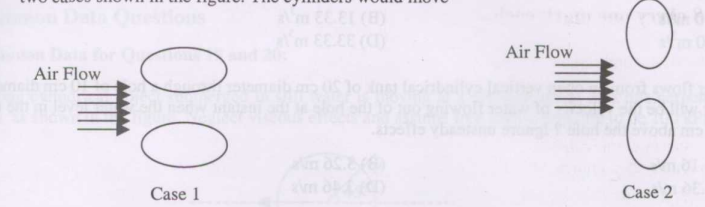
\includegraphics[width=0.5\linewidth]{figs/fig1.png}
    \caption*{}
    \label{fig:Q 20}
\end{figure}
\begin{enumerate}
 
    \item away from each other for Case 1 and towards each other for Case 2
    \item towards each other for Case 1 and away from each other for Case 2
    \item away from each other for Case 1 and away from each other for Case 2
    \item towards each other for Case 1 and towards each other for Case 2
\end{enumerate}    




\item A 40 cm cubical block slides on oil (viscosity = 0.80 Pa.s), over a large plane horizontal surface. If the oil film between the block and the surface has a uniform thickness of 0.4 mm, what will be the force required to drag the block at 4 m/s? Ignore the end effects and treat the flow as two dimensional.\hfill[GATE XE 2009]
\begin{enumerate}
\begin{multicols}{2}
    \item 1280 N
    \item 1640 N
    \item 1920 N
    \item 2560 N
\end{multicols}
\end{enumerate}



\item For a floating body, $G$, $B$, and $M$ represent the centre of gravity, centre of buoyancy, and the metacentre, respectively. The body will be stable if\hfill[GATE XE 2009]

\begin{enumerate}
\begin{multicols}{2}
    \item $G$ is located above $B$
    \item $B$ is located above $M$
    \item $M$ is located above $B$
    \item $M$ is located above $G$
\end{multicols}
\end{enumerate}



\item A nozzle has inlet and outlet diameters of 10 cm and 5 cm, respectively. If it discharges air at a steady rate of 0.1 m$^3$/s into the atmosphere, the gauge pressure (static) at the nozzle inlet will be\hfill[GATE XE 2009]

\begin{enumerate}
\begin{multicols}{2}
    \item 1.26 kPa
    \item 1.46 kPa
    \item 3.52 kPa
    \item 3.92 kPa
\end{multicols}
\end{enumerate}




\item Consider incompressible flow through a two-dimensional open channel. At a certain section A-A, the velocity profile is parabolic. Neglecting air resistance at the free surface, find the volume flow rate per unit width of the channel.\hfill[GATE XE 2009]
\begin{figure}[H]
    \centering
    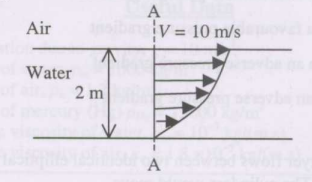
\includegraphics[width=0.5\linewidth]{figs/fig2.png}
    \caption*{}
    \label{fig:Q.24}
\end{figure}
\begin{enumerate}
\begin{multicols}{2}
    \item 10 m$^3$/s
    \item 13.33 m$^3$/s
    \item 20 m$^3$/s
    \item 33.33 m$^3$/s
\end{multicols}
\end{enumerate}




\item Water flows from an open vertical cylindrical tank of 20 cm diameter through a hole of 10 cm diameter. What will be the velocity of water flowing out of the hole at the instant when the water level in the tank is 50 cm above the hole? Ignore unsteady effects.\hfill[GATE XE 2009]
\begin{enumerate}
\begin{multicols}{2}
    \item 3.16 m/s
    \item 3.26 m/s
    \item 3.36 m/s
    \item 3.46 m/s
\end{multicols}
\end{enumerate}





\item In the manometer shown in the figure, the pressure $p_A$ of the gas inside bulb A is approximately.\hfill[GATE XE 2009]
\begin{figure}[H]
    \centering
    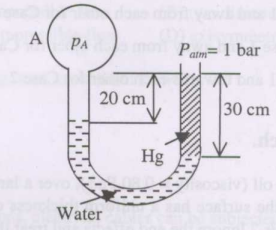
\includegraphics[width=0.5\linewidth]{figs/fig3.png}
    \caption{}
    \label{fig:Q 26}
\end{figure}

\begin{enumerate}
\begin{multicols}{4}
\item 0.8 bar 
\item1.2 bar
\item 1.4 bar
\item1.6 bar 
\end{multicols}
\end{enumerate}



\item Consider a fully developed laminar flow in a circular pipe. If the diameter of the pipe is halved while the flow rate and length of the pipe are kept constant, the head loss increases by a factor of\hfill[GATE XE 2009]

\begin{enumerate}
\begin{multicols}{2}
    \item 4
    \item 8
    \item 16
    \item 32
\end{multicols}
\end{enumerate}



\item A 1:20 model of a submarine is to be tested in a towing tank containing sea water. If the submarine velocity is 6 m/s, at what velocity should the model be towed for dynamic similarity?\hfill[GATE XE 2009]

\begin{enumerate}
\begin{multicols}{2}
    \item 60 m/s
    \item 120 m/s
    \item 180 m/s
    \item 240 m/s
\end{multicols}
\end{enumerate}



\item An oil droplet (density = 800 kg/m$^3$) is rising in still water at a constant velocity of 1 mm/s. Its radius is approximately\hfill[GATE XE 2009]

\begin{enumerate}
\begin{multicols}{2}
    \item 21 micron
    \item 24 micron
    \item 34 micron
    \item 47 micron
\end{multicols}
\end{enumerate}



\item Determine the correctness or otherwise of the following Assertion [a] and the Reason [r]:\hfill[GATE XE 2009]

Assertion [a]: The coefficient of discharge of orifice flow meter is less than that of venturi meter.

Reason [r]: Orifice flow meter is a differential pressure device.

\begin{enumerate}
\begin{multicols}{2}
    \item Both [a] and [r] are true and [r] is the correct reason for [a].
    \item Both [a] and [r] are true but [r] is not the correct reason for [a].
    \item Both [a] and [r] are false.
    \item [a] is true but [r] is false.
\end{multicols}
\end{enumerate}




\item A long cylindrical object submerged in still water is moving at a constant speed of 5 m/s perpendicular to its axis, as shown in the figure. Neglect viscous effects and assume free stream pressure to be 100 kPa.\hfill[GATE XE 2009]
  
  \begin{figure}[H]
      \centering
      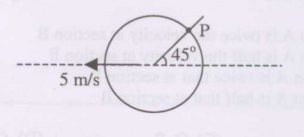
\includegraphics[width=0.5\linewidth]{figs/fig4.png}
      \caption*{}
      \label{fig:Q 31}
  \end{figure}
    




\item The fluid velocity at point P with respect to the cylinder will be approximately\hfill[GATE XE 2009]

\begin{enumerate}[leftmargin=*, itemsep=4pt]
\begin{multicols}{2}
    \item 3.5 m/s
    \item 5 m/s
    \item 7 m/s
    \item 10 m/s
\end{multicols}
\end{enumerate}



\item The absolute pressure at point P will be approximately\hfill[GATE XE 2009]

\begin{enumerate}[leftmargin=*, itemsep=4pt]
\begin{multicols}{2}
    \item 137 kPa
    \item 112 kPa
    \item 87 kPa
    \item 62 kPa
\end{multicols}
\end{enumerate}



\textbf{Common Data for Questions 21 and 22:}

The velocity field for a two dimensional flow is given by:
\begin{align*}
\vec{V}\brak{x, y, t} = -\frac{2x}{t^2}\hat{i} + \frac{y}{t}\hat{j}
\end{align*}

\item The total acceleration is\hfill[GATE XE 2009]

\begin{enumerate}[leftmargin=*, itemsep=4pt]
\begin{multicols}{2}
    \item $-\frac{2x}{t^2}\hat{i}$
    \item $\frac{y}{t^2} \hat{j}$
    \item $-\frac{2x}{t^3}\hat{i}$
    \item $-\frac{y}{t} \hat{j}$
\end{multicols}
\end{enumerate}



\item The given velocity field is\hfill[GATE XE 2009]

\begin{enumerate}[leftmargin=*, itemsep=4pt]
\begin{multicols}{2}
    \item incompressible and rotational
    \item compressible and rotational
    \item incompressible and irrotational
    \item compressible and irrotational
\end{multicols}
\end{enumerate}




\textbf{Linked Answer Questions:}

Statement for Linked Answer Questions 23 and 24:

An incompressible fluid is passed through a T-junction supported on wheels, as shown in the figure. The area at outlet A is twice that of outlet B. While the incoming mass flow rate is fixed, the distribution of flow at the two outlets can be varied by a suitable mechanism built in the system. Assume that the flexible tube offers no resistance to motion, and frictional effects in the pipes and wheels can be neglected. Now, consider the following two cases:

Case 1: The flow rates at sections A and B are equal.
Case 2: The velocities at sections A and B are equal.


\begin{figure}[H]
    \centering
    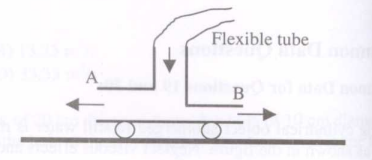
\includegraphics[width=0.5\linewidth]{figs/fig5.png}
    \caption*{}
    \label{fig:Q 36,37}
\end{figure}

\item Which of the following statements are true?\hfill[GATE XE 2009]

P: In Case 1, the velocity at section A is twice the velocity at section B.\\
Q: In Case 1, the velocity at section A is half the velocity at section B.\\
R: In Case 2, the flow rate at section A is twice that at section B.\\
S: In Case 2, the flow rate at section A is half that at section B.
\begin{enumerate}
    

\begin{multicols}{2}
 \item  P, R

 \item P, S

 \item  Q, R

 \item  Q, S
\end{multicols}
\end{enumerate}


\item Which of the following statements are true?\hfill[GATE XE 2009]

P: In Case 1, the system moves to the left.\\
Q: In Case 1, the system moves to the right.\\
R: In Case 2, the system moves to the left.\\
S: In Case 2, the system moves to the right.
\begin{enumerate}
\begin{multicols}{2}
\item P, R

\item P, S

\item Q, R

\item Q, S
\end{multicols}
\end{enumerate}



\begin{tabular}{|c|c|c|}
     \hline
     \textbf{Mineral} & \textbf{Modal abundance \brak{\%}} & \textbf{Partition coefficient}\\
     \hline
     Clinopyroxene & $45$ & $0.506$ \\
      \hline
      Orthopyroxene & $40$ & $0.42$ \\
      \hline
      Olivine & $10$ & $0.045$ \\
      \hline
      Plagioclase & $05$ & $0.019$ \\
      \hline
\end{tabular}







\item Equal size spherical balls when packed together will yield maximum theoretical packing of\hfill[GATE XE 2009]

\begin{multicols}{2}
\begin{enumerate}
    \item 52\%
    \item 68\%
    \item 74\%
    \item 86\%
\end{enumerate}
\end{multicols}



\item Steel containing 0.8\% carbon cooled under equilibrium conditions from molten state to room temperature is soft, because it consists of lamellae of\hfill[GATE XE 2009]

\begin{multicols}{2}
\begin{enumerate}
    \item Ferrite and cementite
    \item Ferrite and austenite
    \item Ferrite and bainite
    \item Ferrite and martensite
\end{enumerate}
\end{multicols}



\item Line broadening in X-ray diffraction pattern occurs on account of\hfill[GATE XE 2009]

\begin{multicols}{2}
\begin{enumerate}
    \item Coarse crystallite size
    \item Residual stresses
    \item Multiplicity of phases
    \item Coring of crystallites
\end{enumerate}
\end{multicols}




\item Inter-granular corrosion of austenitic stainless steel is promoted by\hfill[GATE XE 2009]

\begin{multicols}{2}
\begin{enumerate}
    \item Fine grained microstructure
    \item Coarse grained microstructure
    \item Soaking steel at 700$^\degree$C in air
    \item Quenching from 1000$^\degree$C
\end{enumerate}
\end{multicols}



\item Ferrites are preferred materials for use in high frequency applications (GHz range) as opposed to other ferromagnetic materials because ferrites also have\hfill[GATE XE 2009]

\begin{multicols}{2}
\begin{enumerate}
    \item High permeability
    \item High electrical resistivity
    \item High saturation magnetisation
    \item Low coercivity
\end{enumerate}
\end{multicols}



\item During indirect intra-band transition, electrons undergo\hfill[GATE XE 2009]

\begin{multicols}{2}
\begin{enumerate}
    \item Change in energy and momentum
    \item Change in momentum but no change in energy
    \item Change neither in energy nor in momentum
    \item Change in energy but no change in momentum
\end{enumerate}
\end{multicols}



\item A material has a band gap of 2.4 eV. Which of the following wavelengths of light will it absorb?\hfill[GATE XE 2009]

\begin{multicols}{2}
\begin{enumerate}
    \item 700 nm
    \item 550 nm
    \item 650 nm
    \item 400 nm
\end{enumerate}
\end{multicols}



\item Thermal conductivity of a material at a temperature greater than Debye temperature\hfill[GATE XE 2009]

\begin{multicols}{2}
\begin{enumerate}
    \item Is independent of temperature
    \item Decreases inversely with temperature
    \item Increases linearly with temperature
    \item Increases exponentially with temperature
\end{enumerate}
\end{multicols}






\item  Match the following classes of materials given in Column I with the electron spin alignments in atoms shown in Column II.\hfill[GATE XE 2009]



\noindent
Match the roles shown in Column I with those shown in Column II.

\begin{tabular}{@{}p{0.35\textwidth}p{0.35\textwidth}@{}}
\textbf{Column I} & \textbf{Column II} \\
P. Ferromagnetic & 1. $\uparrow\downarrow\uparrow\downarrow$ \\
Q. Anti-ferromagnetic & 2. $\rightarrow \nearrow \searrow\swarrow\swarrow \leftarrow$ \\
R. Ferrimagnetic & 3. $\uparrow\uparrow\uparrow\uparrow$ \\
S. Paramagnetic & 4. $\downarrow\downarrow\downarrow\downarrow$ \\
& 5. $\uparrow\uparrow\uparrow$ \\
\end{tabular}



\begin{enumerate}
\begin{multicols}{2}

\item P-3, Q-1, R-4, S-5 
\item P-4, Q-2, R-5, S-3 
\item P-3, Q-1, R-5, S-2  
\item P-3, Q-2, R-4, S-1 
\end{multicols}
\end{enumerate}



\item Match the following \textbf{experimental techniques} given in Column I with applications given in Column II.
\hfill[GATE XE 2009]


\begin{tabular}{p{7cm} p{6cm}}
\textbf{Column I} & \textbf{Column II} \\
P. Differential Scanning Calorimetry & 1. Dislocation studies \\
Q. Atomic Absorption Spectroscopy & 2. Surface Topography \\
R. Scanning Electron Microscopy & 3. Electrical Conductivity \\
S. Transmission Electron Microscopy & 4. Trace Element Analysis \\
& 5. Phase Transformation \\
\end{tabular}



\noindent
(A) P-5, Q-4, R-2, S-1 \quad
(B) P-5, Q-1, R-3, S-2 \\
(C) P-2, Q-5, R-3, S-1 \quad
(D) P-1, Q-5, R-4, S-2
\item Match the following materials given in Column I with their applications given in Column II.\hfill[GATE XE 2009]



\begin{tabular}{p{6cm} p{6cm}}
\textbf{Column I} & \textbf{Column II} \\
P. Nylon & 1. Electrical switch housing \\
Q. Urea formaldehyde & 2. Conducting polymers \\
R. Polyaniline & 3. Heating Element \\
S. Alumina & 4. Gears for toys \\
& 5. Polishing material \\
\end{tabular}



\noindent
(A) P-2, Q-4, R-3, S-5 \hfill
(B) P-4, Q-1, R-2, S-5 \\
(C) P-3, Q-4, R-2, S-1 \hfill
(D) P-4, Q-5, R-3, S-2


\item Match the following materials given in Column I with their applications given in Column II.\hfill[GATE XE 2009]



\begin{tabular}{p{6cm} p{6cm}}
\textbf{Column I} & \textbf{Column II} \\
P. Silicon carbide fibre & 1. Fibre glass boat \\
Q. Polyester fibre & 2. Heating element \\
R. Thoria doped tungsten & 3. Magnetic material \\
S. Nichrome & 4. Electric bulb filament \\
& 5. Armour material \\
\end{tabular}



\begin{enumerate}
    

\item  P-5, Q-1, R-3, S-2 
\item P-5, Q-3, R-2, S-1 
\item P-5, Q-1, R-4, S-2
 \item P-1, Q-5, R-4, S-2 
\end{enumerate}

\item Correlate the material properties given in Column I with the units given in Column II.\hfill[GATE XE 2009]



\begin{tabular}{p{6cm} p{6cm}}
\textbf{Column I} & \textbf{Column II} \\
P. Magnetic moment & 1. MN$^{-\tfrac{3}{2}}$ \\
Q. Thermal conductivity & 2. H m$^{-1}$ \\
R. Fracture toughness & 3. A m$^2$ \\
S. Electron mobility & 4. m$^2$ V$^{-1}$ s$^{-1}$ \\
& 5. J s$^{-1}$ m$^{-1}$ K$^{-1}$ \\
\end{tabular}



\begin{enumerate}
    \item 

 \item -3, Q-2, R-4, S-1
 \item -2, Q-5, R-1, S-4
 \item -4, Q-5, R-1, S-3
 \item -3, Q-5, R-1, S-4

\end{enumerate}

\item A simply supported beam with an overhanging end is loaded as shown below. The maximum bending moment in the beam is\hfill[GATE XE 2009]

\begin{multicols}{2}
\begin{enumerate}
    \item 2 kN m
    \item 1 kN m
    \item 0.75 kN m
    \item 0.25 kN m
\end{enumerate}
\end{multicols}



\item A body $ P $ while moving rectilinearly with velocity $ v_0 $ collides directly with another body $ Q $, which is at rest, as shown below. Assuming both the bodies have the same mass and the collision is elastic, the velocities of the bodies after the collision, measured positive towards right, are\hfill[GATE XE 2009]

\begin{multicols}{2}
\begin{enumerate}
    \item $v_p = -\frac{v_0}{2},\; v = \frac{v_0}{2}$
    \item $v_p = \frac{v_0}{2},\; v = \frac{v_0}{2}$
    \item $v_p = 0,\; v = \frac{v_0}{2}$
    \item $v_p = 0,\; v = v_0$
\end{enumerate}
\end{multicols}



\item A stepped circular shaft, fixed at one end, is subjected to two axial forces as shown below. The maximum tensile stress in the shaft is\hfill[GATE XE 2009]

\begin{multicols}{2}
\begin{enumerate}
    \item 120 MPa
    \item 210 MPa
    \item 153 MPa
    \item 390 MPa
\end{enumerate}
\end{multicols}



\item A thin string of negligible mass with one end fixed to the roof is wound around a circular disc of radius 2 m and mass 10 kg, as shown below. The disc rolls vertically down under the action of its own weight. Considering acceleration due to gravity as 10 m/s$^2$, the tension in the string is\hfill[GATE XE 2009]

\begin{multicols}{2}
\begin{enumerate}
    \item 0 N
    \item 25.0 N
    \item 33.3 N
    \item 50 N
\end{enumerate}
\end{multicols}

\item {Molecular weight distribution of a polystyrene polymer and the number fraction of polymer chains in the molecular weight range are given below.}\hfill[GATE XE 2009]

\begin{table}[htbp]
  \centering
  \caption{Table-3}
  \label{table3}
  \begin{tabular}{cc}
  \textbf{Processing Technique} & \textbf{Producct} \\ \\
    P. Calendering & 1. Pipes \\
    Q. Extrusion & 2. Disposable cups \\
    R. Injection moulding & 3. Sheets \\
    S. Thermoforming & 4. Nylon gears \\
  \end{tabular}
\end{table}



The number average molecular weight and the number average degree of polymerization will be

\begin{enumerate}
    

    \item 15.750 kg/mol and 151
    \item 21.350 kg/mol and 203
    \item15.750 kg/mol and 302
    \item 21.350 kg/mol and 205
\end{enumerate}


\textbf{Common Data for Question 55 and 56}
\item The change in the thickness of the plate is\hfill[GATE XE 2009]
\begin{multicols}{2}
\begin{enumerate}
    \item 2.39 
    \item 5.25 
    \item 7.12 
    \item 9.16 
\end{enumerate}
\end{multicols}



\item The change in the surface area of the plate is\hfill[GATE XE 2009]
\begin{multicols}{2}
\begin{enumerate}
    \item 9.72 mm\textsuperscript{2}
    \item 13.61 mm\textsuperscript{2}
    \item 17.52 mm\textsuperscript{2}
    \item 24.50 mm\textsuperscript{2}
\end{enumerate}
\end{multicols}



\textbf{Common Data for Question 57 and 58}

\item The maximum shear stress due to torsion in the length PQ is\hfill[GATE XE 2009]
\begin{multicols}{2}
\begin{enumerate}
    \item 15.75 MPa
    \item 21.22 MPa
    \item 30.56 MPa
    \item 51.21 MPa
\end{enumerate}
\end{multicols}

\item  The rotation of the free end S due to the torsion is\hfill[GATE XE 2009]
\begin{multicols}{2}
\begin{enumerate}
    \item 0.25$^\degree$
    \item 0.58$^\degree$
    \item 1.22$^\degree$
    \item 1.25$^\degree$
\end{enumerate}
\end{multicols}



\textbf{Common Data for Question 59 and 60}

\item The maximum compression of the spring is\hfill[GATE XE 2009]
\begin{multicols}{2}
\begin{enumerate}
    \item 2 mm
    \item 20.2 mm
    \item 202.0 mm
    \item 2020 mm
\end{enumerate}
\end{multicols}



\item In the ensuing Simple Harmonic Motion of the body, the magnitude of maximum acceleration is\hfill[GATE XE 2009]
\begin{multicols}{2}
\begin{enumerate}
    \item 100 m/s\textsuperscript{2}
    \item 200 m/s\textsuperscript{2}
    \item 500 m/s\textsuperscript{2}
    \item 1000 m/s\textsuperscript{2}
\end{enumerate}
\end{multicols}




\item A small spherical ball fails at a normal load of 10 kN under the arrangement as shown below. The vertical force $F$ required to crush the ball is\hfill[GATE XE 2009]
\begin{figure}[H]
    \centering
    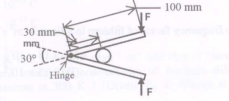
\includegraphics[width=0.5\linewidth]{figs/fig6.png}
    \caption*{}
    \label{fig:Q 62}
\end{figure}

    (A) 11.6 kN \hfill
    (B) 6.0 kN \hfill
   (C) 3.5 kN \hfill
   (D) 3.1 kN




\noindent
\item A projectile is fired from point P at an angle of $45^\degree$ with horizontal as shown below. If $g$ is acceleration due to gravity, then the speed required to reach a point Q lying on the horizontal surface at a distance of $R$ from point P is\hfill[GATE XE 2009]

\begin{figure}[H]
    \centering
    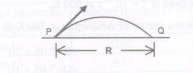
\includegraphics[width=0.5\linewidth]{figs/fig7.png}
    \caption*{}
    \label{fig:Q 63}
\end{figure}

   (A)  $\sqrt{Rg/2}$  \hfill
   (B)  $\sqrt{Rg}$  \hfill
    (C)$\sqrt{2Rg}$  \hfill 
    (D) $\sqrt{3Rg}$ \hfill




\noindent
\item The state of stress at a point in a loaded body is given as $\sigma_x = +40$ MPa, $\sigma_y = +60$ MPa, $\tau_{xy} = +10$ MPa. The sum of the principal stresses at that point is\hfill[GATE XE 2009]

     (A)+20 MPa \hfill
     (B)+50 MPa  \hfill
     (C)+100 MPa \hfill
    (D) +110 MPa




\noindent
\item A composite system of two metal bars, as shown below, is made of two dissimilar materials having areas of cross section $A_1$ and $A_2$, Young's moduli $E_1$ and $E_2$ and coefficients of thermal expansion $\alpha_1$ and $\alpha_2$. If the temperature of the system is raised by $\Delta T$, then the resultant axial force required to be applied to the rigid end plates to maintain the same length $L$ is\hfill[GATE XE 2009]
\begin{figure}[H]
    \centering
    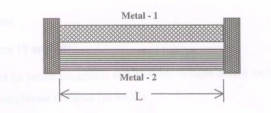
\includegraphics[width=0.5\linewidth]{figs/fig8.png}
    \caption*{}
    \label{fig:Q 65}
\end{figure}
\begin{enumerate}

    \item $(E_1 \alpha_1 A_1 + E_2 \alpha_2 A_2) \Delta T$
    \item $\left(\frac{1}{E_1 A_1} + \frac{1}{E_2 A_2} \right)^{-1} \Delta T$
    \item $(E_1 + E_2)\brak{\alpha_1 + \alpha_2}\brak{A_1 + A_2} \Delta T$
    \item $(E_1 A_1 + E_2 A_2) \Delta T$
 
\end{enumerate}

\item The state of stress at a point is as shown below. Both the normal and shear stresses on a plane, inclined at an angle of $45^\degree$ with horizontal are zero. If $\sigma_x = \sigma_y = 200$ MPa, the shear stress $T_{xy}$ is\hfill[GATE XE 2009]

  \begin{figure}[H]
       \centering
       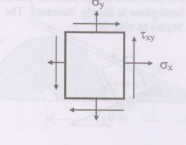
\includegraphics[width=0.5\linewidth]{figs/fig9.png}
       \caption*{}
       \label{fig:Q 66}
   \end{figure} 

\begin{multicols}{2}
\begin{enumerate}
    \item 50 MPa
    \item 70 MPa
    \item 100 MPa
    \item 200 MPa
\end{enumerate}
\end{multicols}



\bigskip
\item A simply supported beam of span $L$ and flexural rigidity $EI$ carries a uniformly distributed load $w$ per unit length. The deflection at the mid-span of the beam is\hfill[GATE XE 2009]
\begin{multicols}{2}
\begin{enumerate}
    \item $\frac{wL^4}{48EI}$
    \item $\frac{5wL^4}{384EI}$
    \item $\frac{5wL^4}{96EI}$
    \item $\frac{3wL^4}{16EI}$
\end{enumerate}
\end{multicols}



\item During plastic impact of two bodies, which of the following statements is correct?\hfill[GATE XE 2009]
\begin{multicols}{2}
\begin{enumerate}
    \item Both energy and momentum are conserved
    \item Energy is not conserved; momentum is conserved
    \item Energy is conserved; momentum is not conserved
    \item Neither energy nor momentum is conserved
\end{enumerate}
\end{multicols}




\item A disc of radius 1 m is rolling on the ground without slip. At a certain instant the center of the disc is moving with a velocity of 10 m/s and an acceleration of $a = + 10$ m/s$^2$. The magnitude of acceleration of point $P$ on the disc instantaneously touching the ground is\hfill[GATE XE 2009]

\begin{figure}[H]
    \centering
    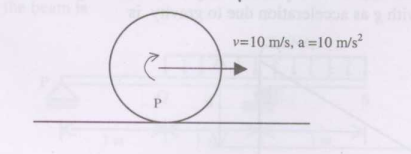
\includegraphics[width=0.5\linewidth]{figs/fig10.png}
    \caption*{}
    \label{fig:Q 69}
\end{figure}


\begin{multicols}{2}
\begin{enumerate}
    \item 0.0 m/s$^2$
    \item 10.0 m/s$^2$
    \item 20.0 m/s$^2$
    \item 100.0 m/s$^2$
\end{enumerate}
\end{multicols}



\item A block of length $a$ and height $b$ rests on a rough inclined plane (coefficient of friction $\mu$). The angle $\alpha$ of the inclined plane is slowly increased. The condition that the block will topple due to its own weight before it begins to slide is\hfill[GATE XE 2009]

\begin{figure}[H]
    \centering
    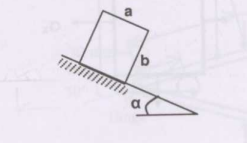
\includegraphics[width=0.5\linewidth]{figs/fig11.png}
    \caption*{}
    \label{fig:70}
\end{figure}
\begin{multicols}{2}
\begin{enumerate}
    \item $\alpha < \mu \frac{b}{a}$
    \item $\alpha > \mu \frac{b}{a}$
    \item $\alpha > \sqrt{1-\mu^2} \frac{b}{a}$
    \item $\alpha < \sqrt{1-\mu^2} \frac{b}{a}$
\end{enumerate}
\end{multicols}




\item A particle enters a smooth frictionless circular loop of radius $R$ at point $P$. If $g$ is acceleration due to gravity, the minimum speed required to complete one full circular revolution is \hfill[GATE XE 2009]
\begin{figure}[H]
    \centering
    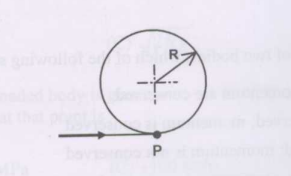
\includegraphics[width=0.5\linewidth]{figs/fig12.png}
    \caption*{}
    \label{fig:Q 71}
\end{figure}

\begin{multicols}{2}
\begin{enumerate}
    \item $\sqrt{5Rg}$
    \item $\sqrt{3Rg}$
    \item $\sqrt{2Rg}$
    \item $\infty$
\end{enumerate}
\end{multicols}




\item A circular cylinder of radius $r$ and mass $m$, starting from the top of an inclined plane, rolls down without slip. After its center moves to a point with vertical height $h$, the velocity of the center of mass is (using $g$ for gravity)\hfill[GATE XE 2009] 
\begin{figure}[H]
    \centering
    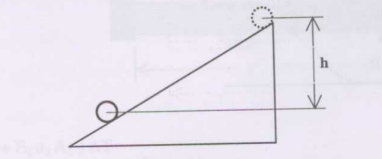
\includegraphics[width=0.5\linewidth]{figs/fig13.png}
    \caption*{}
    \label{fig:Q 72}
\end{figure}

\begin{multicols}{2}
\begin{enumerate}
    \item $\sqrt{3gh}$
    \item $\sqrt{2gh}$
    \item $\sqrt{\frac{4gh}{3}}$
    \item $\sqrt{\frac{3gh}{16}}$
\end{enumerate}
\end{multicols}




\item Rod PQ, hinged at Q, touches a semicircular cylinder at point P. If the cylinder moves with a constant velocity of 10 m/s horizontally, the angular velocity $\omega$ of rod PQ is\hfill[GATE XE 2009] 

\begin{figure}[H]
    \centering
    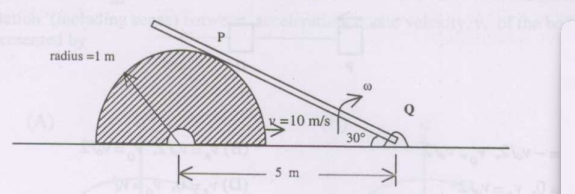
\includegraphics[width=0.5\linewidth]{figs/fig14.png}
    \caption*{}
    \label{fig:Q 73}
\end{figure}
\begin{multicols}{2}
\begin{enumerate}
    \item 0.5 rad/s
    \item 1.15 rad/s
    \item 2.0 rad/s
    \item 2.3 rad/s
\end{enumerate}
\end{multicols}

\item An L-shaped elastic member with flexural rigidity $EI$ is loaded as shown below:
Total strain energy in the member due to bending is:\hfill[GATE XE 2009]

\begin{figure}[H]
    \centering
    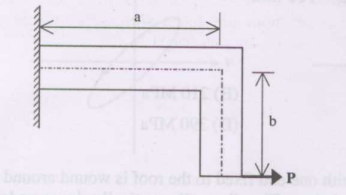
\includegraphics[width=0.5\linewidth]{figs/fig15.png}
    \caption*{}
    \label{fig:Q 74}
\end{figure}
  
   

\begin{multicols}{2}
\begin{enumerate}
    \item $\frac{P^2 b^2 (b/3 + a)}{2EI}$
    \item $\frac{P^2 b^2 (a/3 + b)}{2EI}$
    \item $\frac{P^2 a^2 (b/3 + a)}{3EI}$
    \item $\frac{P^2 a^2 (a/3 + b)}{3EI}$
\end{enumerate}
\end{multicols}


\bigskip

\item A simply supported beam with an overhanging end is loaded as shown. The maximum bending moment in the beam is:\hfill[GATE XE 200]

\begin{figure}[H]
    \centering
    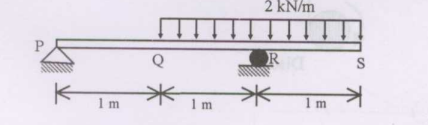
\includegraphics[width=0.5\linewidth]{figs/fig16.png}
    \caption*{}
    \label{fig:Q 75}
\end{figure}
\begin{multicols}{2}
\begin{enumerate}
    \item 2 kN·m
    \item 1 kN·m
    \item 0.75 kN·m
    \item 0.25 kN·m
\end{enumerate}
\end{multicols}




\item A body $P$ moving rectilinearly with velocity $v_0$ collides elastically with a stationary body $Q$, both having the same mass. The velocities after collision (positive to the right) are:\hfill[GATE XE 2009]


\begin{figure}[H]
    \centering
    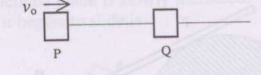
\includegraphics[width=0.5\linewidth]{figs/fig17.png}
    \caption*{}
    \label{fig:Q 76}
\end{figure}
\begin{multicols}{2}
\begin{enumerate}
    \item $v_P = -\frac{v_0}{2}$, $v_Q = \frac{v_0}{2}$
    \item $v_P = \frac{v_0}{2}$, $v_Q = \frac{v_0}{2}$
    \item $v_P = 0$, $v_Q = \frac{v_0}{2}$
    \item $v_P = 0$, $v_Q = v_0$
\end{enumerate}
\end{multicols}




\item A stepped circular shaft fixed at one end is subjected to two axial forces as shown. The maximum tensile stress in the shaft is:\hfill[GATE XE 2009]

\begin{figure}[H]
    \centering
    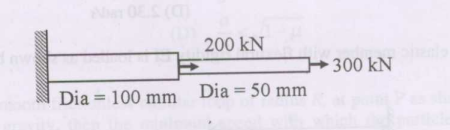
\includegraphics[width=0.5\linewidth]{figs/fig18.png}
    \caption*{}
    \label{fig:Q 77}
\end{figure}
   

\begin{multicols}{2}
\begin{enumerate}
    \item 120 MPa
    \item 210 MPa
    \item 153 MPa
    \item 390 MPa
\end{enumerate}
\end{multicols}



\item A thin string fixed to the roof is wound around a disc of radius 2 m and mass 10 kg, which rolls vertically down under gravity $g=10\,\mathrm{m/s^2}$. The tension in the string is:\hfill[GATE XE 2009]


   \begin{figure}{H}
       \centering
       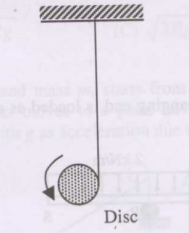
\includegraphics[width=0.5\linewidth]{figs/fig19.png}
       \caption*{}
       \label{fig:Q 78}
   \end{figure}
    

\begin{multicols}{2}
\begin{enumerate}
    \item 0 N
    \item 25.0 N
    \item 33.3 N
    \item 50 N
\end{enumerate}
\end{multicols}




\item A spring-mass system executes simple harmonic motion in vertical direction: $\frac{d^2 y}{dt^2} + \omega^2 y = 0$. The correct relation between acceleration $a$ and velocity $v$ (including direction) is:\hfill[GATE XE 2009]
\begin{multicols}{2}
\begin{enumerate} 
\item 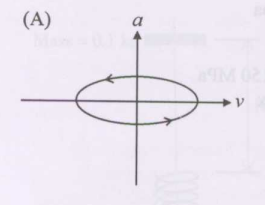
\includegraphics[width=0.4\columnwidth]{figs/fig20.png} 
\item 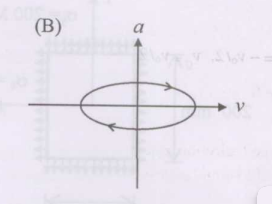
\includegraphics[width=0.4\columnwidth]{figs/fig21.png}
      
\item 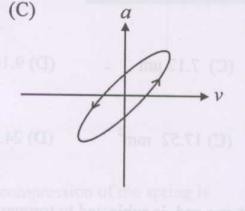
\includegraphics[width=0.4\columnwidth]{figs/fig22.png}   \item 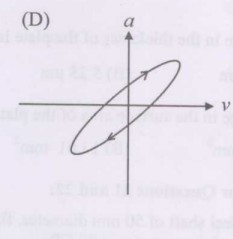
\includegraphics[width=0.4\columnwidth]{figs/fig23.png}
    \\
\end{enumerate}
\end{multicols}


 




\item[] \textbf{(Common Data for Q.79 and Q.80)}  \\
A 10 mm thick steel rectangular plate of size 100 mm $\times$ 200 mm is subjected to biaxial stresses of $\sigma_x = 150$ MPa, $\sigma_y = 200$ MPa, shown below. The Young's modulus and Poisson's ratio are 200 GPa and 0.3 respectively.

\begin{figure}[H]
    \centering
    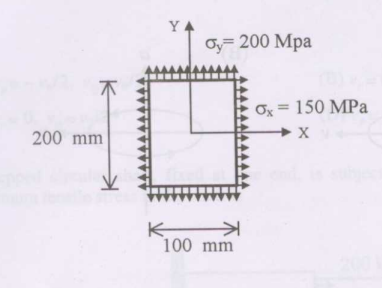
\includegraphics[width=0.5\linewidth]{figs/fig24.png}
    \caption*{}
    \label{fig:Q 79 80}
\end{figure}


     \item The change in the thickness of the plate is\hfill[GATE XE 2009]
\begin{multicols}{2}
\begin{enumerate}
    \item 2.39 $\mu$m
    \item 5.25 $\mu$m
    \item 7.12 $\mu$m
    \item 9.16 $\mu$m

\end{enumerate}
\end{multicols}

\item The change in the surface area of the plate is\hfill[GATE XE 2009]
\begin{multicols}{2}
\begin{enumerate}
    \item 9.72 mm$^2$
    \item 13.61 mm$^2$
    \item 17.52 mm$^2$
    \item 24.50 mm$^2$
\end{enumerate}
\end{multicols}




  
\textbf{(Common Data for Q.81 and Q.82)}  \\
A solid circular steel shaft of 50 mm diameter, fixed at one end, is subjected to torques as shown below. The shearing modulus of the material is 80 GPa. \\


   \begin{figure}[H]
        \centering
        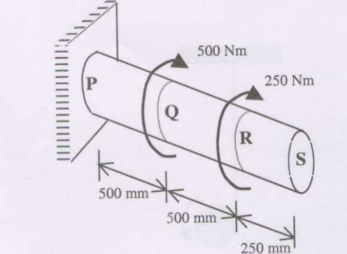
\includegraphics[width=0.5\linewidth]{figs/fig25.png}
        \caption*{}
        \label{fig:Q 81 82}
    \end{figure} 
    
  


\item The maximum shear stress due to torsion in the length PQ is\hfill[GATE XE 2009]
\begin{multicols}{2}
\begin{enumerate}
    \item 15.75 MPa
    \item 21.22 MPa
    \item 30.56 MPa
    \item 51.21 MPa
\end{enumerate}
\end{multicols}

\item The rotation of the free end S due to the torsion is\hfill[GATE XE 2009]
\begin{multicols}{2}
\begin{enumerate}
    \item 0.25$^\degree$
    \item 0.58$^\degree$
    \item 1.22$^\degree$
    \item 1.25$^\degree$
\end{enumerate}
\end{multicols}





\Large\textbf{ Linked Answer Questions}\\
 \textbf{( Statement for Linked Answer Questions Q.83 and Q.84)}  \\

A body of mass 0.1 kg is dropped from a height of 10 m above a spring of stiffness 500 N/m as shown below. The spring is initially in uncompressed natural state. The impact is without any energy loss and the body gets attached to the spring. The acceleration due to gravity is 10 m/s$^2$.\\\\\\\\\\\\\\\\\\\

\begin{figure}[H]
    \centering
    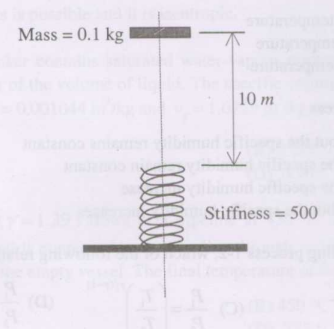
\includegraphics[width=0.5\linewidth]{figs/fig26.png}
    \caption*{}
    \label{fig:Q 83 84}
\end{figure}

\item The maximum compression of the spring is\hfill[GATE XE 2009]
\begin{multicols}{2}
\begin{enumerate}
    \item 2 mm
    \item 20.2 mm
    \item 202.0 mm
    \item 2020 mm
\end{enumerate}
\end{multicols}

\item In the ensuing Simple Harmonic Motion of the body, the magnitude of maximum acceleration is\hfill[GATE XE 2009]
\begin{multicols}{2}
\begin{enumerate}
    \item 100 m/s$^2$
    \item 200 m/s$^2$
    \item 500 m/s$^2$
    \item 1000 m/s$^2$ 
  
    \end{enumerate}
      \end{multicols}
   



\item The ideal gas law is valid for\hfill[GATE XE 2009]
\begin{multicols}{2}
\begin{enumerate}
    \item inert gases
    \item gases at high pressure and high temperature
    \item gases at low pressure and low temperature
    \item gases at low pressure and high temperature
\end{enumerate}
\end{multicols}



\item During the adiabatic saturation process\hfill[GATE XE 2009]
\begin{multicols}{2}
\begin{enumerate}
    \item the relative humidity increases but the specific humidity remains constant
    \item both the relative humidity and the specific humidity remain constant
    \item both the relative humidity and the specific humidity increase
    \item the relative humidity decreases but the specific humidity increases
\end{enumerate}
\end{multicols}



\item For an ideal gas undergoing a throttling process 1--2, which of the following relationships holds?
\hfill[GATE XE 2009]
\begin{multicols}{2}
\begin{enumerate}
    \item $T_1 = T_2$
    \item $\dfrac{P_1}{T_1} = \dfrac{P_2}{T_2}$
    \item $\dfrac{P_1}{T_1} = \dfrac{P_2}{T_2^{\gamma/(\gamma - 1)}}$
    \item $\dfrac{P_1}{T_1} = \dfrac{P_2}{T_2}$
\end{enumerate}
\end{multicols}



\item  A Carnot refrigerator operating between $-1^\degree$ \text{C} and $33^\degree$ \text{C} has a cooling capacity of 1.6 kW. The power consumed by the refrigerator is\hfill[GATE XE 2009]
\begin{multicols}{2}
\begin{enumerate}
    \item 160 W
    \item 178 W
    \item 200 W
    \item 1.8 kW
\end{enumerate}
\end{multicols}



\item An ideal gas undergoes expansion according to the process $PV^{0.5} = \text{constant}$. The temperature of the gas during the expansion process\hfill[GATE XE 2009]
\begin{multicols}{2}
\begin{enumerate}
    \item does not change
    \item increases
    \item decreases
    \item changes depending on the initial condition
\end{enumerate}
\end{multicols}



\item  Air ($\gamma=1.4$) is compressed ideally from an initial state of 1 bar and 300 K to a final temperature of 600 K. The value of the final pressure in bar is\hfill[GATE XE 2009]
\begin{multicols}{2}
\begin{enumerate}
    \item 2
    \item 3.7
    \item 7.2
    \item 11.3
\end{enumerate}
\end{multicols}



\item  On a T-s diagram, the slope of the constant volume line for an ideal gas is\hfill[GATE XE 2009]
\begin{multicols}{2}
\begin{enumerate}
    \item less than that of constant pressure line
    \item more than that of constant pressure line
    \item less than that of constant enthalpy line
    \item equal to that of constant enthalpy line
\end{enumerate}
\end{multicols}



\item  The thermal efficiency of an ideal Rankine cycle is less than that of a Carnot cycle operating between the same maximum and minimum temperature limits, because\hfill[GATE XE 2009]
\begin{multicols}{2}
\begin{enumerate}
    \item heat addition does not take place at constant temperature
    \item the expansion process is not reversible and adiabatic
    \item heat rejection does not take place at constant temperature
    \item the compression process is not reversible and adiabatic
\end{enumerate}
\end{multicols}



\item Atmospheric air (R = 287 J/kg; $\gamma = 1.4$) at 1 bar and 25 °C is compressed adiabatically to 2 bar and 105 °C. Which of the following statements is correct?\hfill[GATE XE 2009]
\begin{multicols}{2}
\begin{enumerate}
    \item The process is possible but irreversible.
    \item The process is possible and reversible.
    \item The process is impossible.
    \item The process is possible and it is isentropic.
\end{enumerate}
\end{multicols}



\item A pressure cooker contains saturated water-vapour mixture at 100 °C with vapour volume eight times that of liquid. Given specific volumes of saturated liquid and vapour at 100 °C as $v_f=0.001044\,m^3/kg$ and $v_g=1.6729\,m^3/kg$ respectively, the quality of the mixture is\hfill[GATE XE 2009]
\begin{multicols}{2}
\begin{enumerate}
    \item 0.005
    \item 0.125
    \item 0.889
    \item 0.995
\end{enumerate}
\end{multicols}



\item An ideal gas ($\gamma=1.39$) flows in a pipeline at 450 °C and 20 bar. A rigid, insulated and initially evacuated vessel is connected to the pipeline through a valve. The valve is opened and the gas fills the vessel. The final temperature of the gas in the vessel is\hfill[GATE XE 2009]
\begin{multicols}{2}
\begin{enumerate}
    \item 247 °C
    \item 450 °C
    \item 625 °C
    \item 732 °C
\end{enumerate}
\end{multicols}



\item An equi-molar mixture of nitrogen ($\gamma=1.4$) and helium ($\gamma=1.67$) initially at 5 bar and 300 °C is expanded adiabatically to 2 bar. The final temperature of the mixture is\hfill[GATE XE 2009]
\begin{multicols}{2}
\begin{enumerate}
    \item 149 °C
    \item 200 °C
    \item 250 °C
    \item 524 °C
\end{enumerate}
\end{multicols}



\item A heat engine $E_1$ operates between an infinite reservoir at 800 °C and a body $B$. The temperature of $B$ remains constant at 550 °C. Heat transferred to the engine $E_1$ is 900 kJ with work output 200 kJ. Another engine $E_2$ operates between $B$ and the atmosphere at 27 °C. Heat rejected to atmosphere is 350 kJ. The thermal efficiency of engine $E_2$ is\hfill[GATE XE 2009]
\begin{multicols}{2}
\begin{enumerate}
    \item 0.39
    \item 0.5
    \item 0.61
    \item 0.635
\end{enumerate}
\end{multicols}



\item A gas turbine power plant operates with air ($\gamma=1.4$) between 1 bar and 20 bar. The maximum thermal efficiency (in \%) for the corresponding air-standard cycle is\hfill[GATE XE 2009]
\begin{multicols}{2}
\begin{enumerate}
    \item 30
    \item 36.7
    \item 48.2
    \item 57.5
\end{enumerate}
\end{multicols}



\item The saturation pressures of water at 100 °C and 105 °C are 101.3 kPa and 120.8 kPa respectively. Given molecular weight of water = 18, the latent heat of water in kJ/kg at 102.5 °C is approximately\hfill[GATE XE 2009]
\begin{multicols}{2}
\begin{enumerate}
    \item 2290
    \item 1250
    \item 820
    \item 330
\end{enumerate}
\end{multicols}



\item An engine reversibly receives 1200 J of heat at 900 K and rejects heat to ambient at 300 K, developing 600 J of work. The irreversibility (in Joules) is\hfill[GATE XE 2009]
\begin{multicols}{2}
\begin{enumerate}
    \item 600
    \item 400
    \item 200
    \item zero
\end{enumerate}
\end{multicols}



\item Saturated liquid water at 0.4 MPa and 1000 kg/hr of steam at 0.4 MPa and 300 °C enter steadily into an insulated mixing chamber. At 0.4 MPa, enthalpies of saturated liquid and saturated vapour are 604.73 and 2738.53 kJ/kg respectively; enthalpy of superheated steam at 300 °C is 3066.75 kJ/kg. The quality of the water-vapour mixture exiting the chamber is 0.9. The mass flow rate of saturated liquid water (kg/hr) is\hfill[GATE XE 2009]
\begin{multicols}{2}
\begin{enumerate}
    \item 182
    \item 282
    \item 382
    \item 1000
\end{enumerate}
\end{multicols}



\item A gas undergoes the polytropic process $PV^{1.3} = \text{constant}$, from initial state 1.5 MPa and 0.09 %m^3% to final pressure of 7.5 MPa. The work done by the gas (kJ) is\hfill[GATE XE 2009]
\begin{multicols}{2}
\begin{enumerate}
    \item -217
    \item -200
    \item 200
    \item 217
\end{enumerate}
\end{multicols}


\section*{Common Data Questions}

\textbf{Common Data for Questions 103 and 104}

Saturated water vapour enters an adiabatic turbine at 0.8 MPa and leaves at 0.1 MPa. The mass flow rate of water vapour is 25 kg/s. Use the following data table to answer the questions 19 and 20.


\begin{center}
\begin{tabular}{|c|c|c|}
    \hline
    Task & Task time (Seconds) & Immediate predecessor(s) \\
    \hline
    P & 20 & - \\ \hline
    Q & 25 & P \\  \hline
    R & 10 & Q \\ \hline
    S & 15 & Q \\ \hline 
    T & 25 & R, S \\    \hline
\end{tabular}
\end{center}


\item The steam quality at turbine exit after isentropic expansion is\hfill[GATE XE 2009]
\begin{multicols}{2}
\begin{enumerate}
    \item 0.47
    \item 0.72
    \item 0.88
    \item 0.94
\end{enumerate}
\end{multicols}



\item If the steam leaves the turbine as saturated vapor, the power produced by the turbine (kW) is\hfill[GATE XE 2009]
\begin{multicols}{2}
\begin{enumerate}
    \item 1640
    \item 2030
    \item 2340
    \item 8830
\end{enumerate}
\end{multicols}



\textbf{Common Data for Question 105 and 106}\\ thev flow rate of Refrigerant R-12 flow rate is 0.03 kg/s. Entering compressor saturated vapor at 150.9 kPa. After adiabatic compression, superheated vapor at 500 kPa and 100 °C enters condenser. Leaves condenser saturated liquid at same pressure.Use the following table to answer the Question 21 and 22.
\begin{table}[h!]
\centering
\begin{tabular}{|c|c|c|c|}
\hline
\textbf{Pressure} & \textbf{Temperature} & \multicolumn{2}{c|}{\textbf{Specific enthalpy}} \\ \cline{3-4} 
\textbf{(kPa)} & \textbf{($^\circ$C)} & $h_f$ (kJ/kg) & $h_g$ (kJ/kg) \\ \hline
150.9 & $-20$ & 17.82 & 178.74 \\ \hline
500 & 15.6 & 50.64 & 195.01 \\ \hline
\end{tabular}
\end{table}

\noindent
For the superheated vapour at 500 kPa and 100$^\degree$C, $h = 252.05$ kJ/kg.

\item The refrigeration effect in kW is\hfill[GATE XE 2009]
\begin{multicols}{2}
\begin{enumerate}
    \item 1.71
    \item 3.84
    \item 4.33
    \item 4.83
\end{enumerate}
\end{multicols}



\item The actual power input to the compressor (kW) is\hfill[GATE XE 2009]
\begin{multicols}{2}
\begin{enumerate}
    \item 0.49
    \item 0.99
    \item 1.71
    \item 2.2
\end{enumerate}
\end{multicols}


\section*{Linked Answer Questions}

\textbf{Statement for Linked Answer Questions 107 and 108:}

An insulated vertical cylinder encloses 0.1 kg of argon (Ar) with the help of a frictionless non-conducting piston as shown in the figure. The mass of the piston is 5 kg and it initially rests on the bottom of the cylinder. The cylinder is connected to a nitrogen (N$_2$) tank at 100 bar through a pipeline fitted with a valve. The valve is opened and nitrogen is slowly admitted into the cylinder. During this operation, the piston is lifted through a height of 10 cm by the nitrogen gas. The initial pressure and temperature of argon gas are 100 kPa and 300 K respectively. The final temperature of argon is 320 K. For argon, $C_p = 520$ J/kgK and $C_v = 312$ J/kgK.

\begin{figure}[H]
    \centering
    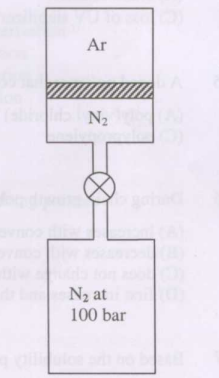
\includegraphics[width=0.5\linewidth]{figs/fig27.png}
    \caption*{}
    \label{fig: Q 107 108}
\end{figure}
     
    



\item Work done by argon during process (kJ) is\hfill[GATE XE 2009]
\begin{multicols}{2}
\begin{enumerate}
    \item 10
    \item 1.041
    \item -0.624
    \item -1.041
\end{enumerate}
\end{multicols}



\item Work done by nitrogen during the process (kJ) is\hfill[GATE XE 2009]
\begin{multicols}{2}
\begin{enumerate}
    \item 1.046
    \item 0.629
    \item -1.046
    \item -10
\end{enumerate}
\end{multicols}


    \item Which of the following trends is the most appropriate for a thixotropic fluid?\hfill[GATE XE 2009]
    \begin{multicols}{2}
    \begin{enumerate}
        \item Viscosity increases with increase in the rate of shear. 
        \item Viscosity increases with increase in the time of application of shear. 
        \item Viscosity decreases with increase in the time of application of shear. 
        \item Viscosity increases with decrease in the rate of shear.
    \end{enumerate}
    \end{multicols}

   \item The temperature at which thermoforming is best carried out is\hfill[GATE XE 2009]
   \begin{multicols}{2}
    \begin{enumerate}
        \item softening temperature 
        \item melting temperature 
        \item glass transition temperature 
        \item 10\% above melting temperature
    \end{enumerate}
    \end{multicols}

    \item  Which of the following blends is immiscible?\hfill[GATE XE 2009]
    \begin{multicols}{2}
    \begin{enumerate}
        \item SAN / PMMA 
        \item PE / PP 
        \item PC / PS 
        \item PET / PBT
    \end{enumerate}
    \end{multicols}

   \item A flexible garden hose pipe made of PVC was observed to get hardened after a length of time. The observation is most likely due to\hfill[GATE XE 2009]
   \begin{multicols}{2}
    \begin{enumerate}
        \item chain scission 
        \item loss of plasticizer 
        \item loss of UV stabilizer 
        \item loss of thermal stabilizer
    \end{enumerate}
    \end{multicols}

    \item A doped polymer that conducts electricity is\hfill[GATE XE 2009]
    \begin{multicols}{2}
    \begin{enumerate}
        \item poly(vinyl chloride) 
        \item polyethylene 
        \item polypropylene 
        \item polypyrrole
    \end{enumerate}
    \end{multicols}

   \item During chain growth polymerization, the molecular weight of the polymer
    \hfill[GATE XE 2009]
   \begin{multicols}{2}
    \begin{enumerate}
        \item increases with conversion 
        \item decreases with conversion 
        \item does not change with conversion 
        \item first increases and then decreases with conversion
    \end{enumerate}
    \end{multicols}

   \item  Based on the solubility parameter ($\delta$), the best solvent for polyethylene ($\delta = 16.2$ MPa$^{1/2}$) is\hfill[GATE XE 2009]
   \begin{multicols}{2}
    \begin{enumerate}
        \item tetrahydrofuran ($\delta = 20.3$ MPa$^{1/2}$) 
        \item toluene ($\delta = 18.3$ MPa$^{1/2}$) 
        \item acetone ($\delta = 19.9$ MPa$^{1/2}$)
        \item methanol ($\delta = 29.7$ MPa$^{1/2}$)\
    \end{enumerate}
    \end{multicols}

    \item  For any polymer, the number average molecular weight ($M_n$), weight average molecular weight ($M_w$) and viscosity average molecular weight ($M_v$), in general, obey the following relationship:\hfill[GATE XE 2009]
    \begin{multicols}{2}
    \begin{enumerate}
        \item $M_n > M_w > M_v$ 
        \item $M_w > M_v > M_n$ 
        \item $M_w > M_n > M_v$ 
        \item $M_v > M_w > M_n$
\end{enumerate}
\end{multicols}







\item Pair the items in the Column I with those in the Column II. 

\hfill[GATE XE 2009]
\begin{minipage}{0.45\textwidth}
\textbf{Column I (Processing step)}
\begin{itemize}
  \item[P.] rotational molding
  \item[Q.] extrusion
  \item[R.] reaction injection molding
  \item[S.] blow molding
\end{itemize}
\end{minipage}
\hfill
\begin{minipage}{0.45\textwidth}
\textbf{Column II (Item)}
\begin{itemize}
  \item[1.] polyurethane
  \item[2.] use of a gas
  \item[3.] centrifugal force
  \item[4.] twin screw
\end{itemize}
\end{minipage}


\begin{multicols}{2}
\begin{enumerate}
\item P-3, Q-1, R-2, S-4
\item P-2, Q-4, R-3, S-1
\item P-4, Q-2, R-1, S-3
\item P-3, Q-4, R-1, S-2
\end{enumerate}
\end{multicols}

\item Strain, $\gamma$, in a polymer melt varies with time on application of stress $s$ by the following relation:\hfill[GATE XE 2009]
\[
\eta \frac{d\gamma}{dt} + G\gamma = s
\]
If a steady shear stress, $s_0$, is applied, the strain at the steady state, $\gamma_0$, is given by:\hfill[GATE XE 2009]

\begin{multicols}{2}
\begin{enumerate}
\item $\dfrac{s_0}{G}$
\item $\dfrac{s_0}{\eta}$
\item $s_0 G$
\item $s_0 \eta$
\end{enumerate}
\end{multicols}

\item Match the polymerization initiator with the respective process.\hfill[GATE XE 2009][0.5em]
\begin{minipage}{0.45\textwidth}
\textbf{Initiator}
\begin{itemize}
  \item[P.] benzyl lithium
  \item[Q.] tropolyn chloride
  \item[R.] AIBN
  \item[S.] TiCl$_3$/Al(Et)$_3$
\end{itemize}
\end{minipage}
\hfill
\begin{minipage}{0.45\textwidth}
\textbf{Process}
\begin{itemize}
  \item[1.] coordination polymerization
  \item[2.] anionic polymerization
  \item[3.] cationic polymerization
  \item[4.] radical polymerization
\end{itemize}
\end{minipage}


\begin{multicols}{2}
\begin{enumerate}
\item P-2, Q-3, R-4, S-1
\item P-2, Q-3, R-1, S-4
\item P-3, Q-1, R-2, S-4
\item P-4, Q-2, R-1, S-3
\end{enumerate}
\end{multicols}

\item Arrange the following polyamides (PA) in decreasing order of their melting points:\hfill[GATE XE 2009]

\begin{itemize}
\item[I.] PA 66
\item[II.] PA 6
\item[III.] PA 10
\item[IV.] PA 12
\end{itemize}

\begin{multicols}{2}
\begin{enumerate}
\item IV $>$ I $>$ II $>$ III
\item I $>$ II $>$ III $>$ IV
\item III $>$ II $>$ IV $>$ I
\item II $>$ IV $>$ III $>$ I
\end{enumerate}
\end{multicols}

\item Match the characterization technique with the most appropriate property.\hfill[GATE XE 2009[0.5em]
\begin{minipage}{0.45\textwidth}
\textbf{Characterization Technique}
\begin{itemize}
  \item[P.] infrared spectroscopy
  \item[Q.] thermo-gravimetric analysis
  \item[R.] transmission electron microscopy
  \item[S.] differential scanning calorimetry
\end{itemize}
\end{minipage}
\hfill
\begin{minipage}{0.45\textwidth}
\textbf{Property}
\begin{itemize}
  \item[1.] melting point
  \item[2.] functional group
  \item[3.] degradation temperature
  \item[4.] morphology
\end{itemize}
\end{minipage}


\begin{multicols}{2}
\begin{enumerate}
\item P-3, Q-2, R-4, S-1
\item P-3, Q-4, R-2, S-1
\item P-2, Q-1, R-4, S-3
\item P-2, Q-3, R-4, S-1
\end{enumerate}
\end{multicols}
\item Match the rubber ingredients with their appropriate function.\hfill[GATE XE 2009[0.5em]
\begin{minipage}{0.45\textwidth}
\textbf{Rubber ingredient}
\begin{itemize}
  \item[P.] ZnO
  \item[Q.] salicylic acid
  \item[R.] ester gum
  \item[S.] paraffin oil
\end{itemize}
\end{minipage}
\hfill
\begin{minipage}{0.45\textwidth}
\textbf{Function}
\begin{itemize}
  \item[1.] tackifier
  \item[2.] extender
  \item[3.] accelerator
  \item[4.] retarder
\end{itemize}
\end{minipage}


\begin{multicols}{2}
\begin{enumerate}
\item P-3, Q-4, R-1, S-2
\item P-3, Q-4, R-2, S-1
\item P-4, Q-3, R-2, S-1
\item P-4, Q-3, R-1, S-2
\end{enumerate}
\end{multicols}

\item At the start of a step growth polymerization there are $N_0$ moles of monomer A (molecular weight $M_A$) and $N_0$ moles of monomer B (molecular weight $M_B$). At the end of the polymerization there are $N$ moles of polymer chains. Assuming no condensation product, the number of average molecular weight is\hfill[GATE XE 2009]

\begin{multicols}{2}
\begin{enumerate}
\item $\dfrac{2N_0(M_A + M_B)}{N}$
\item $\dfrac{N_0(M_A + M_B)}{N}$
\item $\dfrac{N_0(M_A + M_B)}{2N}$
\item $\dfrac{N_0^2(M_A + M_B)}{N^2}$
\end{enumerate}
\end{multicols}

\item The ratio of the complex dynamic modulus to the storage modulus of a polymer system with a phase angle of $45^\degree$ is\hfill[GATE XE 2009]

\begin{multicols}{2}
\begin{enumerate}
\item 0
\item $1 - i$
\item $1 + i$
\item $1 \pm i$
\end{enumerate}
\end{multicols}

\item Match the additive to its most common function.\hfill[GATE XE 2009[0.5em]
\begin{minipage}{0.45\textwidth}
\textbf{Additive}
\begin{itemize}
  \item[P.] talc
  \item[Q.] carbon fibre
  \item[R.] dioctyl phthalate
  \item[S.] antimony trioxide
\end{itemize}
\end{minipage}
\hfill
\begin{minipage}{0.45\textwidth}
\textbf{Function}
\begin{itemize}
  \item[1.] plasticizer
  \item[2.] flame retardant
  \item[3.] filler
  \item[4.] reinforcement
\end{itemize}
\end{minipage}


\begin{multicols}{2}
\begin{enumerate}
\item P-3, Q-4, R-2, S-1
\item P-4, Q-3, R-1, S-2
\item P-4, Q-3, R-2, S-1
\item P-3, Q-4, R-1, S-2
\end{enumerate}
\end{multicols}

\item Match the polymer mechanical property with the appropriate testing method.\hfill[GATE XE 2009[0.5em]
\begin{minipage}{0.45\textwidth}
\textbf{Mechanical property}
\begin{itemize}
  \item[P.] flexural strength
  \item[Q.] impact strength
  \item[R.] hardness
  \item[S.] tensile strength
\end{itemize}
\end{minipage}
\hfill
\begin{minipage}{0.45\textwidth}
\textbf{Testing method}
\begin{itemize}
  \item[1.] notched Izod
  \item[2.] Shore-D
  \item[3.] ASTM D 638
  \item[4.] three-point bending
\end{itemize}
\end{minipage}


\begin{multicols}{2}
\begin{enumerate}
\item P-4, Q-1, R-2, S-3
\item P-3, Q-2, R-1, S-4
\item P-3, Q-1, R-2, S-4
\item P-4, Q-1, R-2, S-3
\end{enumerate}
\end{multicols}
\textbf{Common Data Questions}

\textbf{Common Data for Questions 127 and 128:}\\
An aligned short carbon fibre reinforced polyester composite has a fibre content of 40\% by volume. The elastic modulus of carbon fibre and polyester resin are 250 GPa and 35 GPa, respectively. The fibre diameter is $5~\mu m$ and the ultimate tensile strength of the fibre is 1240 MPa.



\item The modulus of the composite is\hfill[GATE XE 2009]
\begin{multicols}{2}
\begin{enumerate}
\item 121 GPa
\item 215 GPa
\item 285 GPa
\item 142.5 GPa
\end{enumerate}
\end{multicols}

\item The fibre-matrix bond strength, assuming a critical fibre length of 12 mm, is\hfill[GATE XE 2009]
\begin{multicols}{2}
\begin{enumerate}
\item 258 MPa
\item 2.58 MPa
\item 25.8 MPa
\item 0.258 MPa
\end{enumerate}
\end{multicols}



\textbf{Common Data for Questions 129 and 130:}\\
A plasticating screw of an injection molding unit injects 0.1 L/s of polymer through a mold, which is a cylindrical tube having a diameter of 20 mm and a length of 100 mm. The pressure drop across the mold is 100 MPa.


\item The shear stress exerted by the polymer on the wall of the mold is\hfill[GATE XE 2009]
\begin{multicols}{2}
\begin{enumerate}
\item 2.5 MPa
\item 10 MPa
\item 5 MPa
\item 1 MPa
\end{enumerate}
\end{multicols}

\item The power consumed by the plasticizing screw is\hfill[GATE XE 2009]
\begin{multicols}{2}
\begin{enumerate}
\item 5 kW
\item 1 kW
\item 2.5 kW
\item 10 kW
\end{enumerate}
\end{multicols}




\textbf{Linked Answer Questions}

\textbf{Statement for Linked Answer Questions 131 and 132:}

The density of a poly(ethylene terephthalate) (PET) sample is $1.407~\text{g/cm}^3$, and the heat of fusion of the sample obtained from differential scanning calorimetry (DSC) is $54.6~\text{J/g}$. The density of the PET crystalline phase is $1.515~\text{g/cm}^3$ and of the PET amorphous phase is $1.335~\text{g/cm}^3$.


\item The fractional crystallinity of the sample is\hfill[GATE XE 2009]
\begin{multicols}{2}
\begin{enumerate}
\item 0.23
\item 0.36
\item 0.40
\item 0.43
\end{enumerate}
\end{multicols}

\item The heat of fusion of the PET crystalline phase is\hfill[GATE XE 2009]
\begin{multicols}{2}
\begin{enumerate}
\item 21.8 J/g
\item 136.5 J/g
\item 68.2 J/g
\item 158.3 J/g
\end{enumerate}
\end{multicols}




\item Among the following amino acids, the one that has a disulfide linkage is\hfill[GATE XE 2009]
\begin{multicols}{2}
\begin{enumerate}
\item (-)-proline
\item (-)-cystine
\item (-)-cysteine
\item (-)-histidine
\end{enumerate}
\end{multicols}

\item The method of packaging of food under sterile environment, after independently sterilizing the food and packing material, is termed as\hfill[GATE XE 2009]
\begin{multicols}{2}
\begin{enumerate}
\item active packaging
\item vacuum packaging
\item flexible packaging
\item aseptic packaging
\end{enumerate}
\end{multicols}

\item Mild heat treatment of food to inactivate enzymes that would otherwise cause its deterioration during frozen storage is termed as\hfill[GATE XE 2009]
\begin{multicols}{2}
\begin{enumerate}
\item stewing
\item blanching
\item boiling
\item pasteurization
\end{enumerate}
\end{multicols}

\item The most suitable evaporator for concentration of fruit juices is\hfill[GATE XE 2009]
\begin{multicols}{2}
\begin{enumerate}
\item agitated film evaporator
\item falling film evaporator
\item long tube evaporator
\item short tube evaporator
\end{enumerate}
\end{multicols}

\item Souring of milk is primarily due to the conversion of lactose to\hfill[GATE XE 2009]
\begin{multicols}{2}
\begin{enumerate}
\item lactobionic acid
\item lactic acid
\item lactol
\item lactonic acid
\end{enumerate}
\end{multicols}

\item The selective media used for isolating \textit{Escherichia coli} is\hfill[GATE XE 2009]
\begin{multicols}{2}
\begin{enumerate}
\item blood agar
\item mannitol salt agar
\item eosin methylene blue agar
\item rose bengal malt extract agar
\end{enumerate}
\end{multicols}

\item A method in which continuous electric current is passed through food to heat it rapidly while maintaining quality is called\hfill[GATE XE 2009]
\begin{multicols}{2}
\begin{enumerate}
\item microwave cooking
\item irradiation
\item ohmic heating
\item sonication
\end{enumerate}
\end{multicols}

\item A cyclone separator is used for the separation of\hfill[GATE XE 2009]
\begin{multicols}{2}
\begin{enumerate}
\item particles from liquid
\item liquid droplets from gas
\item fine particles from gas
\item fine particles from solids
\end{enumerate}
\end{multicols}



\item Match the items in Group I with the most appropriate items in Group II.\hfill[GATE XE 2009]

\begin{minipage}[t]{0.45\textwidth}
\textbf{Group I}
\begin{itemize}
  \item[P.] Tocopherol
  \item[Q.] Myoglobin
  \item[R.] Crocetin
  \item[S.] Catechin
\end{itemize}
\end{minipage}
\hfill
\begin{minipage}[t]{0.45\textwidth}
\textbf{Group II}
\begin{itemize}
  \item[1.] Oxygen binding
  \item[2.] Yellow pigment
  \item[3.] Antioxidant
  \item[4.] Green pigment
  \item[5.] Tanning agent
\end{itemize}
\end{minipage}



\begin{multicols}{2}
\begin{enumerate}
\item P -- 3, Q -- 1, R -- 2, S -- 5
\item P -- 1, Q -- 3, R -- 4, S -- 5
\item P -- 3, Q -- 1, R -- 5, S -- 2
\item P -- 1, Q -- 3, R -- 5, S -- 4
\end{enumerate}
\end{multicols}

\item Two key reactions involved in enzymatic browning of food are
\hfill[GATE XE 2009]
\begin{multicols}{2}
\begin{enumerate}
\item hydroxylation of phenol to \textit{p}-dihydroxybenzene followed by its oxidation to \textit{p}-quinone
\item oxidation of phenol to \textit{p}-quinone followed by its reduction to \textit{p}-dihydroxybenzene
\item oxidation of phenol to \textit{o}-quinone followed by its reduction to \textit{o}-dihydroxybenzene
\item hydroxylation of phenol to \textit{o}-dihydroxybenzene followed by its oxidation to \textit{o}-quinone
\end{enumerate}
\end{multicols}

\item The correct structure of synthetic antioxidant BHT (butylated hydroxy toluene) is\hfill[GATE XE 2009]


\begin{multicols}{2}
\begin{enumerate}
\item 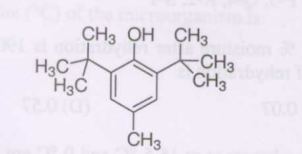
\includegraphics[width=0.5\columnwidth]{figs/fig28.png}
    

\item  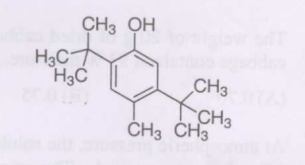
\includegraphics[width=0.5\columnwidth]{figs/fig29.png}
    
\item  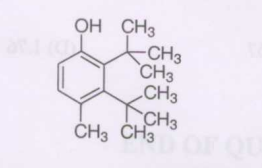
\includegraphics[width=0.5\columnwidth]{figs/fig30.png}
    
\item  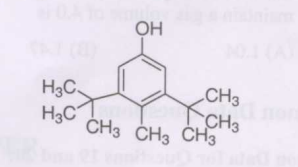
\includegraphics[width=0.5\columnwidth]{figs/fig31.png}
    
\end{enumerate}
\end{multicols}

\item Wet grain was dried from an initial moisture content of 50\% to a final moisture content of 20\% (on wet basis). The amount of moisture removed to get 1000 kg of the final product is\hfill[GATE XE 2009]

\begin{multicols}{2}
\begin{enumerate}
\item 800 kg
\item 200 kg
\item 300 kg
\item 600 kg
\end{enumerate}
\end{multicols}

\item The correct pair of food borne disease and its causative microorganism is\hfill[GATE XE 2009]

\begin{multicols}{2}
\begin{enumerate}
\item Hemorrhagic inflammation of intestinal wall -- \textit{Campylobacter jejuni}
\item Paratyphoid fever -- \textit{Staphylococcus aureus}
\item Typhoid fever -- \textit{Salmonella typhimurium}
\item Listerellosis -- \textit{Leptospira biflexa}
\end{enumerate}
\end{multicols}
\item Fermentation process of vinegar production involves\hfill[GATE XE 2009]

\begin{multicols}{2}
\begin{enumerate}
\item ethanolic fermentation followed by reduction of ethanol
\item direct acetic acid production without ethanolic fermentation
\item anaerobic fermentation of acetone
\item ethanolic fermentation followed by oxidation of ethanol
\end{enumerate}
\end{multicols}

\item In a double pipe heat exchanger the outer diameter of the inner pipe is $d_1$ and the inner diameter of the outer pipe is $d_2$. The equivalent diameter of the annulus for heat transfer is
\hfill[GATE XE 2009]
\begin{multicols}{2}
\begin{enumerate}
\item $(d_1 + d_2)/2$
\item $(d_2^2 - d_1^2)/d_1$
\item $(d_2 - d_1)$
\item $(d_2^2 - d_1^2)/d_2$
\end{enumerate}
\end{multicols}

\item Match various phases of a typical bacterial growth cycle in Group I with most appropriate bacterial activity in Group II.\hfill[GATE XE 2009]

\begin{minipage}[t]{0.45\textwidth}
\textbf{Group I}
\begin{itemize}
  \item[P.] Lag phase
  \item[Q.] Exponential phase
  \item[R.] Stationary phase
  \item[S.] Decline phase
\end{itemize}
\end{minipage}
\hfill
\begin{minipage}[t]{0.45\textwidth}
\textbf{Group II}
\begin{itemize}
  \item[1.] Number of viable cells decreases
  \item[2.] Growth ceases and population remains constant
  \item[3.] Preparatory phase for cell division
  \item[4.] Cells divide steadily at constant rate
  \item[5.] Cells aggregate
\end{itemize}
\end{minipage}



\begin{multicols}{2}
\begin{enumerate}
\item P -- 4, Q -- 3, R -- 2, S -- 1
\item P -- 5, Q -- 4, R -- 1, S -- 2
\item P -- 2, Q -- 1, R -- 3, S -- 4
\item P -- 3, Q -- 4, R -- 2, S -- 1
\end{enumerate}
\end{multicols}

\item The weight of 20 g of dried cabbage containing 5\% moisture after rehydration is 190 g. If the fresh cabbage contained 93\% moisture, the coefficient of rehydration is\hfill[GATE XE 2009]

\begin{multicols}{2}
\begin{enumerate}
\item 0.70
\item 0.75
\item 0.07
\item 0.57
\end{enumerate}
\end{multicols}

\item At atmospheric pressure, the solubilities of CO$_2$ in a beverage at 15.5$^\degree$C and 0$^\degree$C are 1.0 volume and 1.7 volume respectively. The pressure (in atm.) required to carbonate the beverage at 4.5$^\degree$C so as to maintain a gas volume of 4.0 is\hfill[GATE XE 2009]

\begin{multicols}{2}
\begin{enumerate}
\item 1.04
\item 1.47
\item 1.67
\item 1.76
\end{enumerate}
\end{multicols}


\noindent\textbf{Common Data Questions}

\noindent\textbf{Common Data for Questions 19 and 20:}
The partial pressure and vapour pressure of water vapour in air at 27 $^\degree$C and 1 atm. are 0.028 and 0.035 atm respectively. (Molecular weight of air is 29)

\item The humidity of air (kg water /kg air) is\hfill[GATE XE 2009]

\begin{multicols}{2}
\begin{enumerate}
\item 0.0496
\item 0.082
\item 0.018
\item 0.046
\end{enumerate}
\end{multicols}

\item The percentage relative humidity of air is\hfill[GATE XE 2009]

\begin{multicols}{2}
\begin{enumerate}
\item 46
\item 80
\item 20
\item 35
\end{enumerate}
\end{multicols}

\item Fermentation process of vinegar production involves\hfill[GATE XE 2009]

\begin{multicols}{2}
\begin{enumerate}
\item ethanolic fermentation followed by reduction of ethanol
\item direct acetic acid production without ethanolic fermentation
\item anaerobic fermentation of acetone
\item ethanolic fermentation followed by oxidation of ethanol
\end{enumerate}
\end{multicols}

\item In a double pipe heat exchanger the outer diameter of the inner pipe is $d_1$ and the inner diameter of the outer pipe is $d_2$. The equivalent diameter of the annulus for heat transfer is
\hfill[GATE XE 2009]
\begin{multicols}{2}
\begin{enumerate}
\item $(d_1 + d_2)/2$
\item $(d_2^2 - d_1^2)/d_1$
\item $(d_2 - d_1)$
\item $(d_2^2 - d_1^2)/d_2$
\end{enumerate}
\end{multicols}

\item Match various phases of a typical bacterial growth cycle in Group I with most appropriate bacterial activity in Group II.\hfill[GATE XE 2009]

\begin{minipage}[t]{0.45\textwidth}
\textbf{Group I}
\begin{itemize}
  \item[P.] Lag phase
  \item[Q.] Exponential phase
  \item[R.] Stationary phase
  \item[S.] Decline phase
\end{itemize}
\end{minipage}
\hfill
\begin{minipage}[t]{0.45\textwidth}
\textbf{Group II}
\begin{itemize}
  \item[1.] Number of viable cells decreases
  \item[2.] Growth ceases and population remains constant
  \item[3.] Preparatory phase for cell division
  \item[4.] Cells divide steadily at constant rate
  \item[5.] Cells aggregate
\end{itemize}
\end{minipage}


\begin{multicols}{2}
\begin{enumerate}
\item P -- 4, Q -- 3, R -- 2, S -- 1
\item P -- 5, Q -- 4, R -- 1, S -- 2
\item P -- 2, Q -- 1, R -- 3, S -- 4
\item P -- 3, Q -- 4, R -- 2, S -- 1
\end{enumerate}
\end{multicols}

\item The weight of 20 g of dried cabbage containing 5\% moisture after rehydration is 190 g. If the fresh cabbage contained 93\% moisture, the coefficient of rehydration is\hfill[GATE XE 2009]

\begin{multicols}{2}
\begin{enumerate}
\item 0.70
\item 0.75
\item 0.07
\item 0.57
\end{enumerate}
\end{multicols}

\item At atmospheric pressure, the solubilities of CO$_2$ in a beverage at 15.5$^\degree$C and 0$^\degree$C are 1.0 volume and 1.7 volume respectively. The pressure (in atm.) required to carbonate the beverage at 4.5$^\degree$C so as to maintain a gas volume of 4.0 is\hfill[GATE XE 2009]

\begin{multicols}{2}
\begin{enumerate}
\item 1.04
\item 1.47
\item 1.67
\item 1.76
\end{enumerate}
\end{multicols}


\noindent\textbf{Common Data Questions}

\textbf{Common Data for Questions 158 and 159:}


The partial pressure and vapour pressure of water vapour in air at 27{\degree}C and 1 atm. are 0.028 and 0.035 atm respectively. (Molecular weight of air is 29)

\item The humidity of air (kg water /kg air) is\hfill[GATE XE 2009]

\begin{multicols}{2}
\begin{enumerate}
\item 0.0496
\item 0.082
\item 0.018
\item 0.046
\end{enumerate}
\end{multicols}

\item The percentage relative humidity of air is\hfill[GATE XE 2009]

\begin{multicols}{2}
\begin{enumerate}
\item 46
\item 80
\item 20
\item 35
\end{enumerate}
\end{multicols}

\noindent\textbf{Statement for Linked Answer Questions 160 and 161:}

In an ice-cream manufacturing plant, 1450 litres of ice-cream was obtained from 1000 litres of ice-cream mix.
The composition of ice-cream mix was as follows:
Fat: 12.0\%,
Sugar: 15.0\%,
Milk solids not fat: 11.0\%,
Stabilizer \& emulsifier: 0.3\%.

\item Specific gravity of ice-cream mix at 16 $^\degree$C is\hfill[GATE XE 2009]
\begin{enumerate}
    \item 

 \item  1.096
 \item  0.196
 \item  1.906
 \item  0.916
\end{enumerate}
\item Percent over run in the ice-cream was\hfill[GATE XE 2009]
\begin{enumerate}
 \item  35
 \item  50
 \item  40
 \item  45
\end{enumerate}






\noindent\textbf{Linked Answer Questions}

\noindent\textbf{Statement for Linked Answer Questions 162 and 163:}


In an experiment, the thermal death time (TDT) values for a microorganism were obtained as 2.78 minutes and 9.98 minutes at 121.1$^\degree$C and 115.5$^\degree$C, respectively.



\item The z-value ($^\degree$C) of the microorganism is\hfill[GATE XE 2009]

\begin{multicols}{2}
\begin{enumerate}
\item 9.91
\item 9.19
\item 1.99
\item 0.19
\end{enumerate}
\end{multicols}

\item The TDT value (minutes) at 110$^\degree$C is\hfill[GATE XE 2009]

\begin{multicols}{2}
\begin{enumerate}
\item 35.1
\item 25.8
\item 12.9
\item 21.9
\end{enumerate}
\end{multicols}

\end{enumerate}

 \end{document}

